\chapter{Моделирование оптической системы}
\label{ch:zemax}

\section{Базовая система}
\label{sec:basic_system}

В качестве источника излучения был выбран ИК лазерный диод FPL1055T с длиной волны излучения 1550 нм, мощностью излучения в импульсном режиме 300 мВт, поперечной расходимостью 28${}^\circ$ и боковой расходимостью 15${}^\circ$~\cite{LDThorlabs}. Выбранный фотодиод \--- FDGA05 с пиковой длиной волны 1550 нм (регистрируемый диапазон длин волн 800\--1700 нм), фоточувствительностью 0.95 А/Вт, площадью активной области 0.196 мм${}^2$ и материалом сенсора InGaAs~\cite{PDThorlabs}.

Для моделирования оптической системы использовался пакет Zemax OpticStudio 21.1.2. Рассмотрим задание параметров компонентов системы (рисунки~\ref{fig:no_lens_zemax_1}):

\begin{figure}[!h]
    \centering
    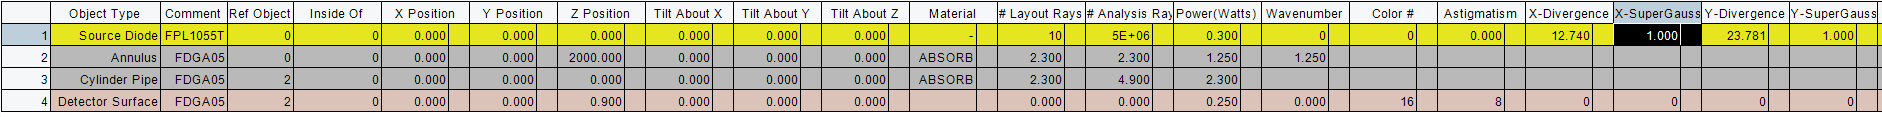
\includegraphics[width=\textwidth]{inc/img/no_lens_1.png}
    \caption{Задание параметров оптической системы в Zemax}
    \label{fig:no_lens_zemax_1}
\end{figure}

\begin{figure}[!h]
    \centering
    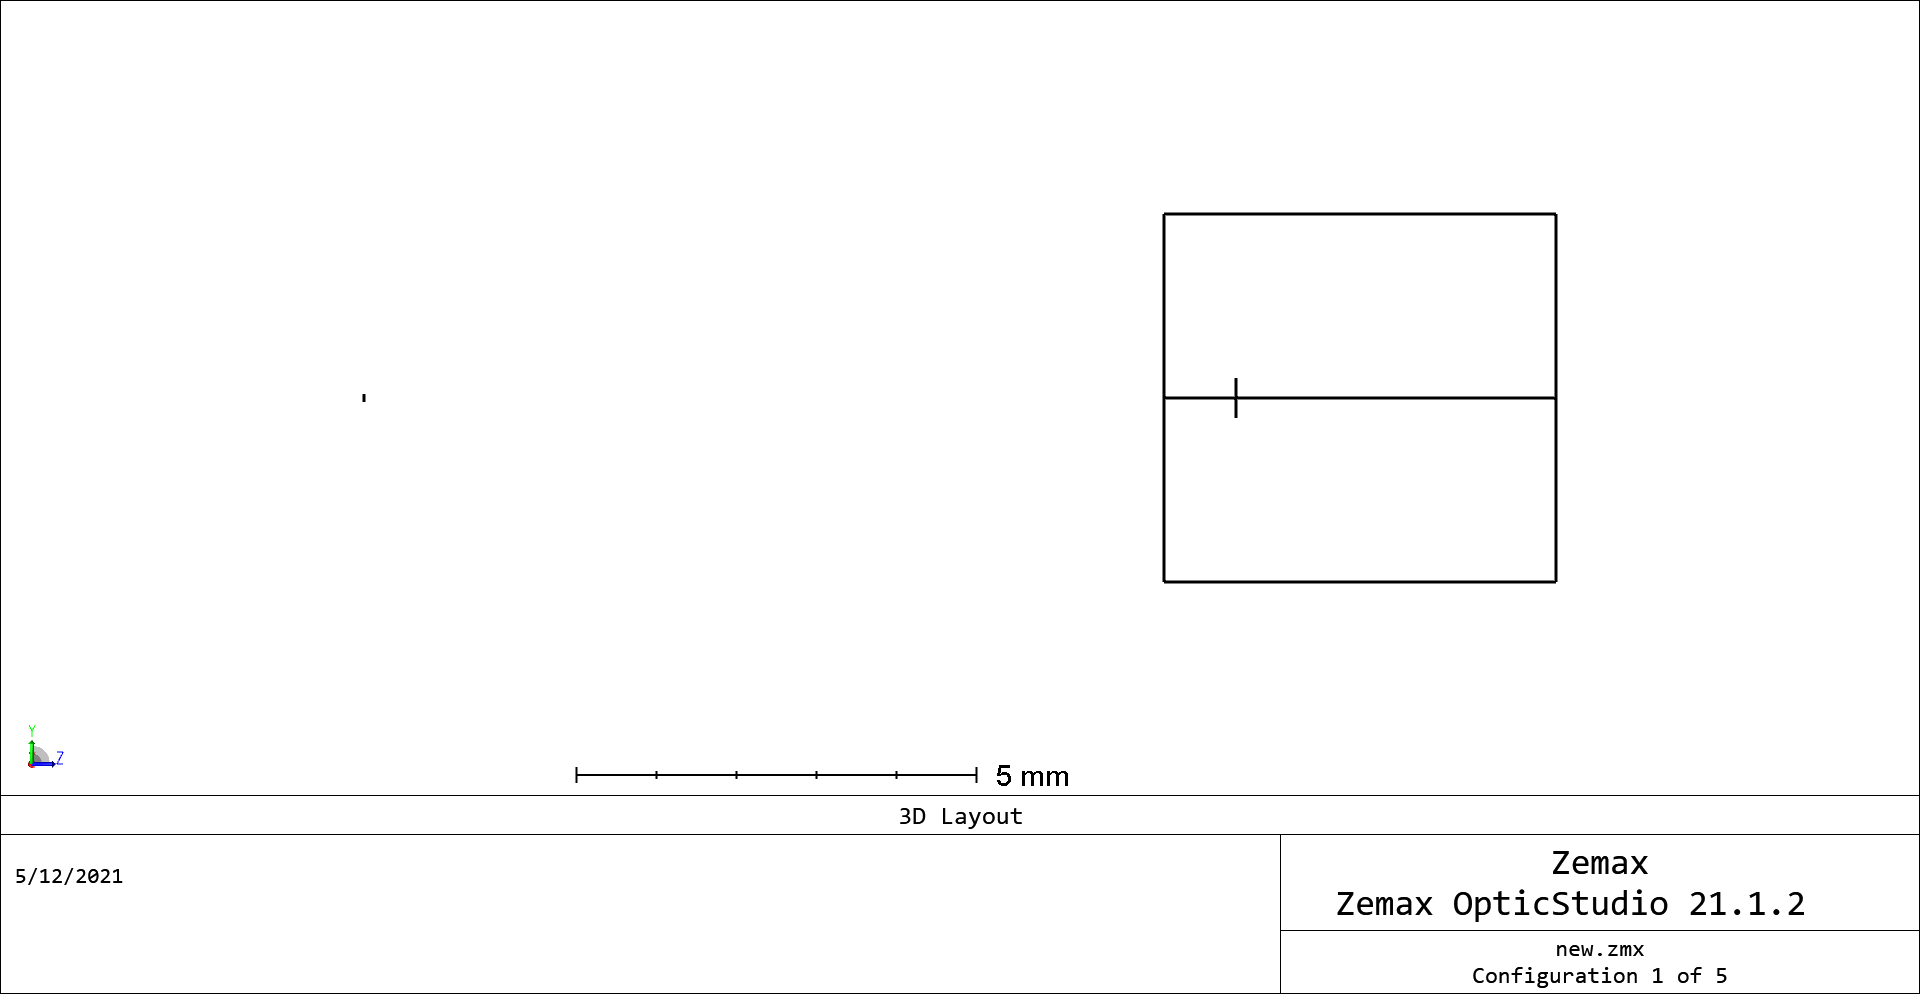
\includegraphics[width=.75\textwidth]{inc/img/layout.png}
    \caption{Вид системы сбоку; слева \--- площадка лазерного диода, справа \--- фотодиод в корпусе; расстояние между лазерным диодом и корпусом фотодиода 10~мм}
    \label{fig:layout}
\end{figure}

Первые 11 колонок (до колонки <<\# Layout Rays>>) универсальны для всех объектов в Zemax: тип объекта, комментарий, референтный объект, нахождение внутри другого объекта, X, Y и Z координаты, наклон вокруг осей X, Y и Z, материал объекта (где применимо). Далее идут специфические для объекта параметры:

Для лазерного диода: количество лучей для рендеринга и для расчётов (выбираются произвольно), мощность источника (выбрана в соответствии с~\cite{LDThorlabs}), номер длины волны (задаётся список используемых длин волн, задана только одна \--- 1550 нм, поэтому в ячейке стоит ноль \--- выбор любой длины волны из списка), цвет лучей на рендере, астигматизм (расстояние, на которое смещено распределение излучения в плоскости XZ), расходимость $\alpha_x$ для направления OX, супер-гауссов коэффициент $G_x$ в направлении OX, расходимость $\alpha_y$ и супер-гауссов коэффициент $G_y$ для направления OY. 

Супер-гауссов коэффициент показывает отличие профиля интенсивности данного пучка от профиля интенсивности Гауссова пучка \--- чем он больше, тем ближе профиль интенсивности излучения к прямоугольному профилю~\cite{Paschotta2008}. Для обоих направлений был выбран супер-гауссов коэффициент $G_{x,y} = 1$ (Гауссово распределение интенсивности). Следуя документации Zemax, можно рассчитать $\alpha_{x,y}$ следующим образом: 

\begin{equation*}
    \alpha_{x, y}=\frac{\theta_{\mathrm{fwhm}}}{\sqrt{2 \ln (2)}},
\end{equation*}

где $\theta_{\mathrm{fwhm}}$ \--- угол расходимости из~\cite{LDThorlabs}.

\begin{figure}[!h]
    \centering
    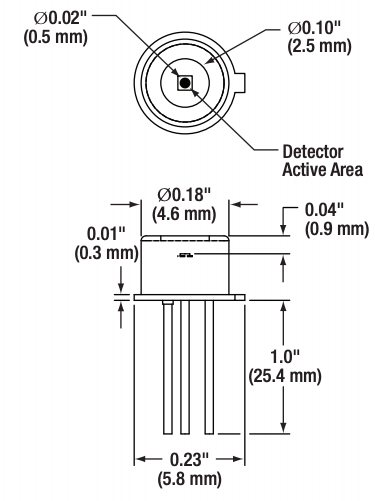
\includegraphics[width=.45\textwidth]{inc/img/pd_size.png}
    \caption{Виды сверху и спереди фотодиода FDGA05~\cite{PDThorlabs}}
    \label{fig:pdviews}
\end{figure}

Два следующих объекта формируют корпус фотодиода: круг с отверстием и трубка. Для круга с отверстием задаются радиусы отверстия и самого круга по большой и малой полуосям. Их значения соответствуют размерам реального лазерного диода~\cite{PDThorlabs}. Его положение задаётся относительно лазерного диода. Для трубки задаются радиусы начала и конца, длина. Радиусы равны и взяты из документации к фотодиоду, длина взята произвольной, положение задаётся относительно круга с отверстием. Этого достаточно для данного моделирования, так как стекло, закрывающее активную область от физического воздействия влияет пренебрежимо слабо на ход лучей и оптическую мощность на приёмнике, а всё, что находится за активной областью не влияет на модель вообще. Виды фотодиода приведены на рисунке~\ref{fig:pdviews}.

Для фотодиода заданы размеры апертуры (взяты из документации), количество угловых и радиальных зон оставлены по умолчанию и необходимы для расчётов в симуляции. Положение фотодиода задаётся относительно круга с отверстием и соответствует положению фотодиода в корпусе. Вид системы сбоку представлен на рисунке~\ref{fig:layout}.

Для анализа системы зададим 5$\cdot \text{10}^6$ лучей, проведём трассировку лучей и получим оптическую мощность, полученную на фотодиоде. Анализ будем производить для различных расстояний между лазерным диодом и фотоприёмником. Результаты всех симуляций приведены в приложении~\ref{ch:simulation_results} в таблице~\ref{tab:distance_simulation}. Построим график зависимости оптической мощности от расстояния (рисунок~\ref{fig:distance_plot}).

\begin{figure}[h]
    \centering
    \begin{minipage}[c]{.49\textwidth}
        \centering
        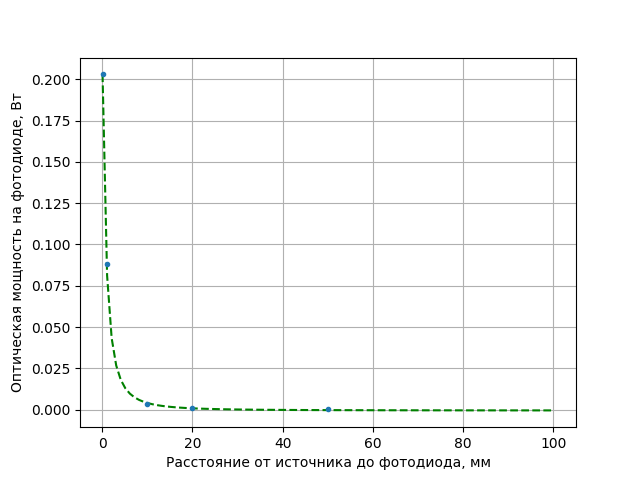
\includegraphics[width=\textwidth]{inc/img/distance.png}
    \end{minipage}
    \hfill
    \begin{minipage}[c]{.49\textwidth}
        \centering
        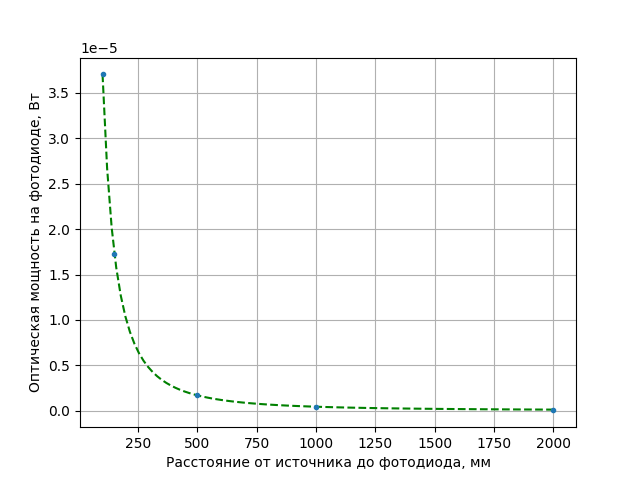
\includegraphics[width=\textwidth]{inc/img/distance2.png}
    \end{minipage}
    \caption{Зависимость оптической мощности на фотодиоде от расстояния между лазерным диодом и фотодиодом: результаты симуляции показаны синими точками, аппроксимирующая функция показана зелёной пунктирной линией}
    \label{fig:distance_plot}
\end{figure}

Эту зависимость можно аппроксимировать функцией $f(x) = \frac{1}{R^2}$, так как зависимость оптической мощности от расстояния подчиняется закону обратных квадратов. Лучшим образом для этого подходит функция $f(x) = \frac{0.615}{(x+1.639)^2} - 2.049\cdot10^{-4}$ (показана на графике пунктирной зелёной линией, результаты симуляции показаны синими точками).

% Аналогично исследуем зависимость оптической мощности от угла расходимости источника при расстоянии между источником и приёмником 100 мм. Выберем одинаковые углы расходимости по обеим осям, так как приёмник симметричен. Результаты симуляции приведены в приложении~\ref{ch:simulation_results} в таблице~\ref{tab:divergence_simulation}. График результатов приведён на рисунке~\ref{fig:divergence_plot}.

% \begin{figure}[h]
%     \centering
%     % This file was created by tikzplotlib v0.9.8.
\begin{tikzpicture}

\definecolor{color0}{rgb}{0.12156862745098,0.466666666666667,0.705882352941177}

\begin{axis}[
tick align=outside,
tick pos=left,
x grid style={white!69.0196078431373!black},
xlabel={Расходимость источника излучения, \(\displaystyle {}^\circ\)},
xmajorgrids,
xmin=-0.45, xmax=31.45,
xminorgrids,
xtick style={color=black},
y grid style={white!69.0196078431373!black},
ylabel={Оптическая мощность на фотодиоде, Вт},
ymajorgrids,
ymin=-0.00056135, ymax=0.01207435,
yminorgrids,
ytick style={color=black}
]
\addplot [semithick, color0, mark=*, mark size=3, mark options={solid}, only marks]
table {%
1 0.0115
3 0.00131
5 0.00047
8 0.000188
10 0.00012
13 7.4e-05
15 5.26e-05
18 3.38e-05
20 2.78e-05
23 2.3e-05
25 1.9e-05
28 1.47e-05
30 1.3e-05
};
\end{axis}

\end{tikzpicture}

%     \caption{Зависимость оптической мощности на фотодиоде от угла расходимости излучения лазерного диода: результаты симуляции показаны синими точками}
%     \label{fig:divergence_plot}
% \end{figure}

\section{Базовая система с собирающей линзой}

Далее добавим в систему собирающую сферическую линзу, конфигурация системы приведена на рисунке~\ref{fig:with_lens_zemax}. 

\begin{figure}[!h]
    \centering
    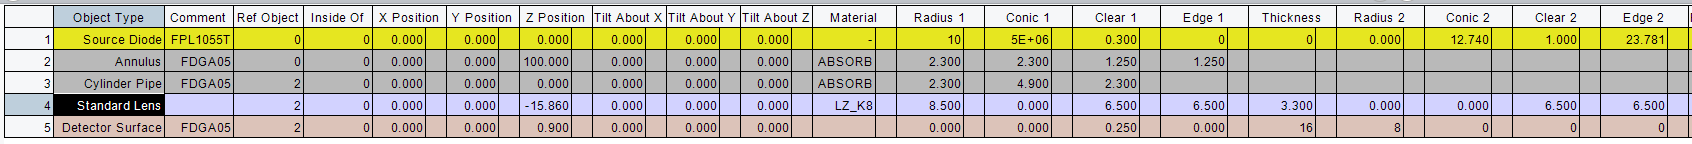
\includegraphics[width=\textwidth]{inc/img/with_lens.png}
    \caption{Задание параметров оптической системы с линзой в Zemax}
    \label{fig:with_lens_zemax}
\end{figure}

\begin{figure}[!h]
    \centering
    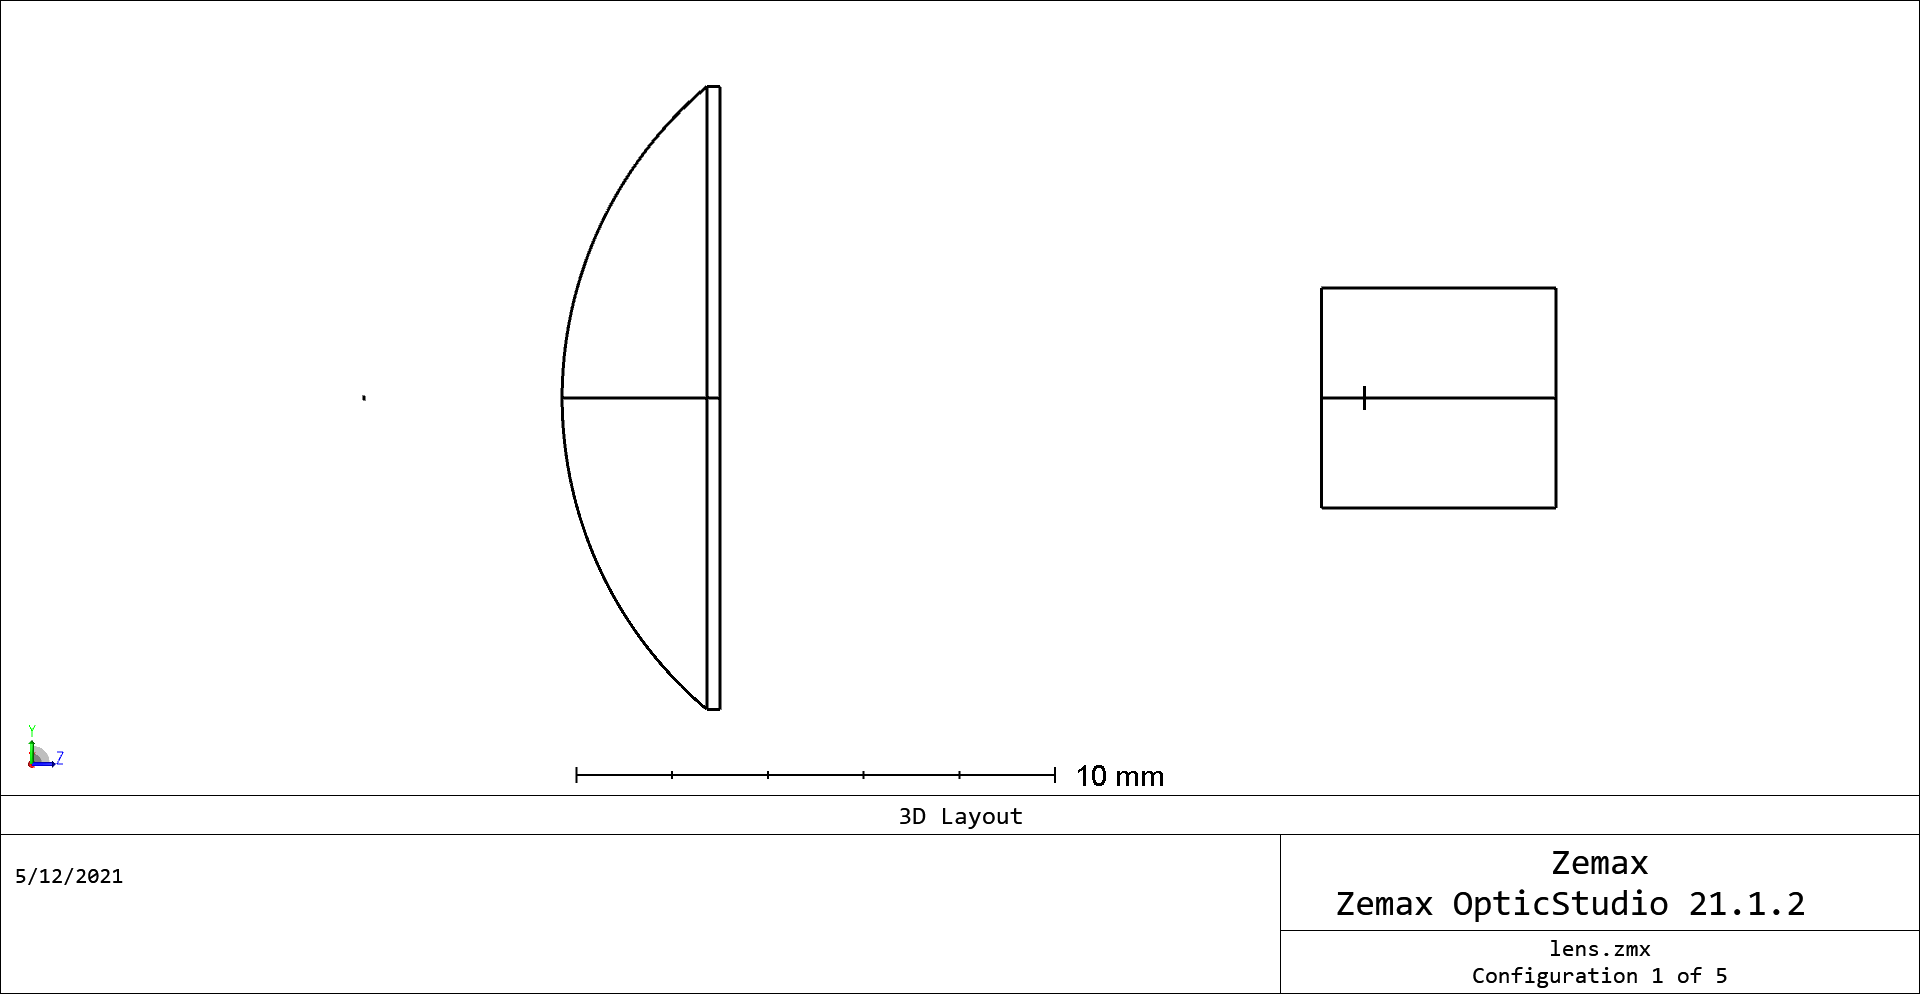
\includegraphics[width=.75\textwidth]{inc/img/layout_lens.png}
    \caption{Вид системы сбоку; слева \--- площадка лазерного диода, по середине \--- собирающая линза, справа \--- фотодиод в корпусе; расстояние между лазерным диодом и корпусом фотодиода 20~мм}
    \label{fig:layout_lens}
\end{figure}


Рассмотрим параметры линзы: зададим положение линзы относительно круга с отверстием, аналогично положению фотодиода. Материал линзы \--- оптическое стекло К8 с показателем преломления $n = 1.507$ на длине волны $\lambda = 1550$ нм. Линза плоско-выпуклая с радиусом кривизны поверхности $R = 8.5$ мм, толщиной линзы $d = 3.3$ мм. Очевидно, что фокусной расстояние этой линзы (по формуле \eqref{eq:focal_length}) $f = 16.76$ мм. 

\begin{equation}
    \frac{1}{f} = \frac{n-1}{R}
    \label{eq:focal_length}
\end{equation}

Тогда для лучшей фокусировки лучей необходимо поместить фотодиод в фокус линзы, то есть необходимо поместить линзу на расстоянии $15.86$ мм от корпуса фотодиода (фотодиод находится на расстоянии $0.9$ мм от поверхности корпуса) \--- рисунок~\ref{fig:with_lens_zemax}. Вид системы с боку представлен на рисунке~\ref{fig:layout_lens}. Аналогично двум предыдущим случаям, будем менять расположение линзы относительно фотодиода и наблюдать за изменением оптической мощности на приёмнике. Все результаты симуляции приведены в приложении~\ref{ch:simulation_results} в таблице~\ref{tab:lens_simulation}. График результатов приведен на рисунке~\ref{fig:lens_plot}.

\begin{figure}[h]
    \centering
    % This file was created by tikzplotlib v0.9.8.
\begin{tikzpicture}

\definecolor{color0}{rgb}{0.12156862745098,0.466666666666667,0.705882352941177}

\begin{axis}[
tick align=outside,
tick pos=left,
x grid style={white!69.0196078431373!black},
xlabel={Расстояние от линзы до фотодиода, мм},
xmajorgrids,
xmin=3.25, xmax=41.75,
xminorgrids,
xtick style={color=black},
y grid style={white!69.0196078431373!black},
ylabel={Оптическая мощность на фотодиоде, Вт},
ymajorgrids,
ymin=-9.571565e-05, ymax=0.00202646265,
yminorgrids,
ytick style={color=black}
]
\addplot [semithick, color0, mark=*, mark size=3, mark options={solid}, only marks]
table {%
5 7.47e-07
10 1.66e-06
15 0.00035
15.86 0.00193
20 0.000437
25 3.32e-05
30 7.06e-06
35 3.52e-06
40 2.3e-06
};
\end{axis}

\end{tikzpicture}

    \caption{Зависимость оптической мощности на фотодиоде от расстояния между собирающей линзой и фотодиодом: результаты симуляции показаны синими точками}
    \label{fig:lens_plot}
\end{figure}

По графику видно, что действительно наибольшая оптическая мощность на фотодиоде наблюдается при нахождении фотодиода в фокусе линзы. 

\section{Исследование диаграммы направленности приёмника}

Для более полного представления о характеристиках фотодиода составим нормированный график оптической мощности в зависимости от направления источника излучения. Для этого заменим лазерный диод на плоский прямоугольный источник (Source Rectangle в Zemax) \--- рисунок~\ref{fig:spinner_zemax}, вид системы с боку приведён на рисунке~\ref{fig:spinner_layout}. 

\begin{figure}[h]
    \centering
    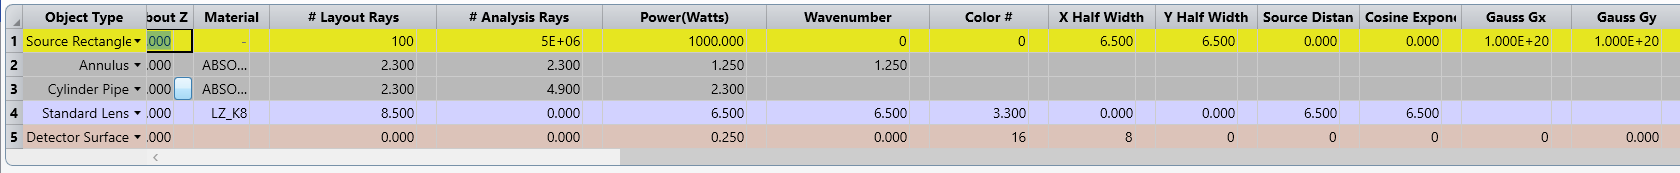
\includegraphics[width=\textwidth]{inc/img/spinner_zemax.png}
    \caption{Задание параметров оптической системы с плоским прямоугольным источником в Zemax}
    \label{fig:spinner_zemax}
\end{figure}

\begin{figure}[!h]
    \centering
    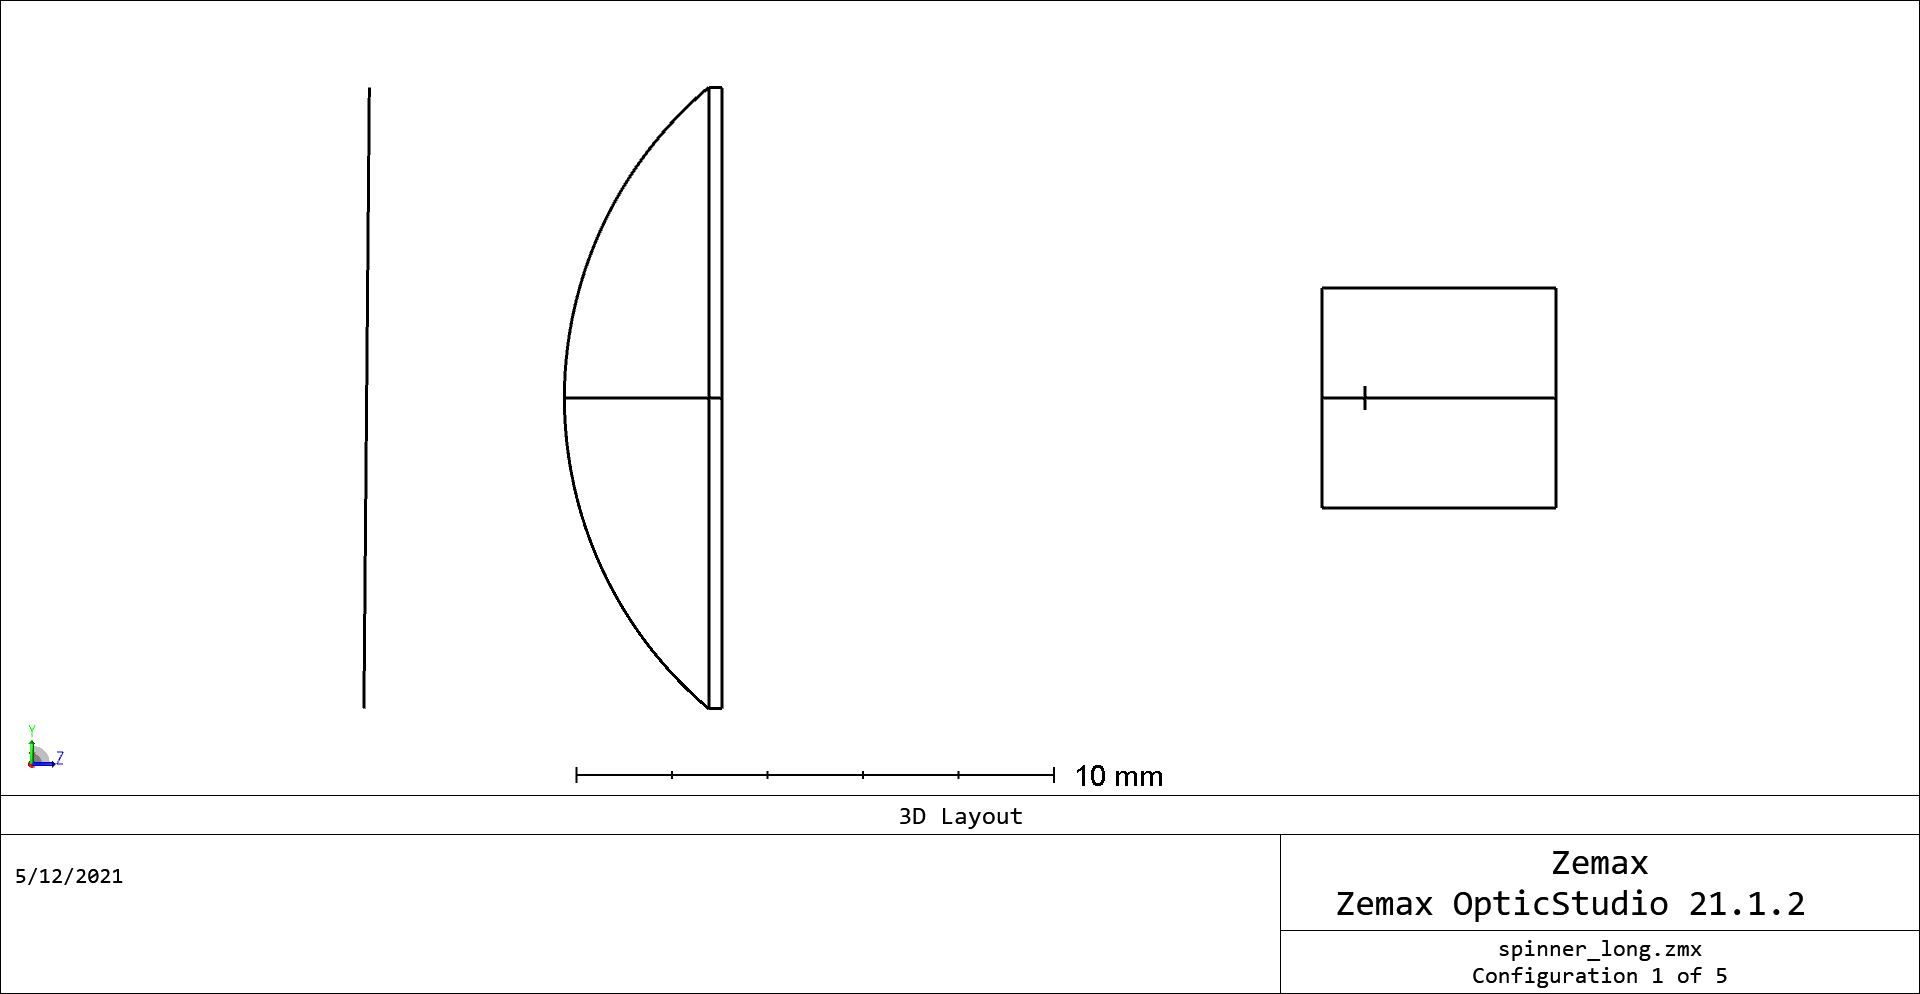
\includegraphics[width=.75\textwidth]{inc/img/spinner_layout.png}
    \caption{Вид системы сбоку; слева \--- площадка плоского источника излучения, справа \--- фотодиод в корпусе; расстояние между лазерным диодом и корпусом фотодиода 20~мм}
    \label{fig:spinner_layout}
\end{figure}

Параметры задаются аналогично параметрам лазерного диода в разделе~\ref{sec:basic_system}. Зададим размеры источника 13x13 мм (квадрат со стороной, равной диаметру линзы). Для создания параллельного пучка излучения зададим супер-гауссовы параметры $G_{x,y}$: чем больше эти параметры, тем более узким выходит пучок. Были выбраны значения $G_{x,y} = 10^{20}$, в результате чего пучок лучей оказывается достаточно параллельным для выбранного расстояния~\cite{Zemax2021}:

\begin{equation}
    I(l, m) \approx I_{0} \exp{\left(-G_{x} l^{2}-G_{y} m^{2}\right)},  G_{x} = G_y \gg l,m \Rightarrow I(l, m) \approx I_0
\end{equation}

где $l$ и $m$ \--- направляющие косинусы вдоль $OX$ и $OY$ соответственно. Величина мощности не важна, так как будем нормировать графики по максимальному значению. Будем вращать источник вокруг $OX$ (в одну сторону, так как система полностью симметрична относительно плоскости $ZOX$; вращаем с шагом в $1^\circ$) и трассировать лучи. Результаты всех симуляций приведены в приложении~\ref{ch:simulation_results} в таблице~\ref{tab:spinner_with_lens}. Построим график зависимости оптической мощности от угла поворота источника (рисунок~\ref{fig:spinner_with_lens_plot}).

\begin{figure}[!h]
    \centering
    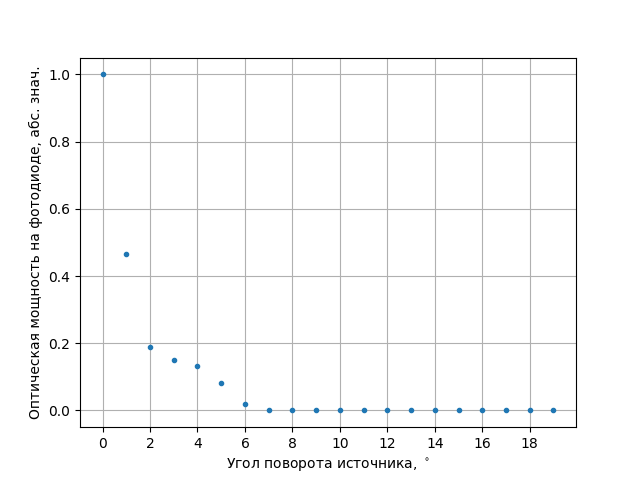
\includegraphics[width=.6\textwidth]{inc/img/spinner_with_lens_plot.png}
    \caption{График зависимости нормированной оптической мощности на приёмнике от угла поворота источника (система с линзой)}
    \label{fig:spinner_with_lens_plot}
\end{figure}

Аналогично проведём моделирование системы без линзы. Результаты всех симуляций приведены в приложении~\ref{ch:simulation_results} в таблице~\ref{tab:spinner_no_lens}, график зависимости оптической мощности от угла поворота источника представлен на рисунке~\ref{fig:spinner_no_lens_plot}.

\begin{figure}[!h]
    \centering
    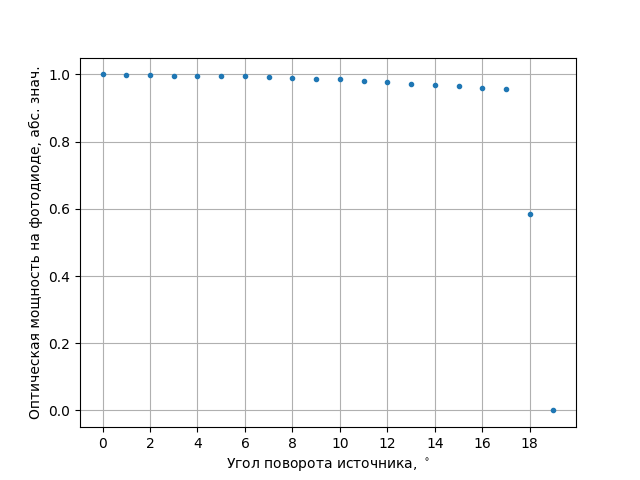
\includegraphics[width=.6\textwidth]{inc/img/spinner_no_lens_plot.png}
    \caption{График зависимости нормированной оптической мощности на приёмнике от угла поворота источника (система без линзы)}
    \label{fig:spinner_no_lens_plot}
\end{figure}

По результатам изменения параметров видно, что самая высокая оптическая мощность достигается при наименьшем расстоянии между фотодиодом и лазерным диодом или при установке собирающей линзы на расстоянии от фотодиода, равном фокусному. Однако даже в наилучших случаях оптическая мощность значительно меньше, чем мощность излучения источника ($0.203$ Вт и $0.00193$ Вт соответственно, против $0.3$ Вт источника). Очевидно, что необходима дополнительная оптическая система для коллимации лучей источника и для фокусировки лучей у приёмника для уменьшения оптических потерь системы и для создания системы, в которой возможно передавать информацию.